% Resumen extendido para el 3rd International Workshop CEDES 2027.
% Formato del resumen extendido del autor sobre el desierto florido.
% Las cifras provienen de ../results/tables/numbers.tex, generado por
% scripts/08_numbers.R desde results/tables.
\documentclass[10pt,a4paper]{article}
\usepackage[utf8]{inputenc}
\usepackage[T1]{fontenc}
\usepackage[spanish,es-tabla,es-nodecimaldot,es-noshorthands]{babel}
\usepackage{lmodern}
\usepackage{microtype}
\usepackage[margin=2cm]{geometry}
\usepackage{graphicx}
\usepackage{booktabs}
\usepackage{parskip}
\usepackage[hidelinks]{hyperref}
\graphicspath{{../results/figures/}}
% Generated by scripts/08_numbers.R - do not edit by hand.
\newcommand{\EarthFluxVersion}{0.1.0.9000}
\newcommand{\EarthFluxCommit}{95d3175}
\newcommand{\Seed}{20270121}
\newcommand{\NMC}{200}
\newcommand{\NTests}{614}
\newcommand{\NExpectations}{4.473}
\newcommand{\NTestsFailed}{0}
\newcommand{\NTestsError}{17}
\newcommand{\NTestsSkipped}{9}
\newcommand{\NTestsPassed}{588}
\newcommand{\NExports}{73}
\newcommand{\NLinesR}{24.027}
\newcommand{\NDecisions}{17}
\newcommand{\VerRows}{49}
\newcommand{\VerVerified}{31}
\newcommand{\VerCorroborated}{3}
\newcommand{\VerCandidate}{9}
\newcommand{\VerDiscrepancies}{7}
\newcommand{\VerFixed}{2}
\newcommand{\SceneElevMax}{863}
\newcommand{\SceneCellsProvince}{3.779}
\newcommand{\SceneCellsValid}{3.653}
\newcommand{\NStations}{63}
\newcommand{\NStationsDMC}{5}
\newcommand{\NStationsINIA}{21}
\newcommand{\NStationsFDF}{35}
\newcommand{\NStationsISD}{2}
\newcommand{\NStationsWind}{7}
\newcommand{\RepStationName}{General Bernardo O'Higgins, Chillán Ad.}
\newcommand{\RepStationDist}{80}
\newcommand{\NCVDays}{90}
\newcommand{\NFolds}{17}
\newcommand{\NCVPred}{51.705}
\newcommand{\CVTaCOneRmse}{2,70}
\newcommand{\CVTaCOneRmseLo}{2,57}
\newcommand{\CVTaCOneRmseHi}{2,84}
\newcommand{\CVTaCOneBias}{-0,16}
\newcommand{\CVTaCOneR}{0,70}
\newcommand{\CVTaCOneFailed}{0}
\newcommand{\CVTaCOneN}{5.498}
\newcommand{\CVTaCOneLapRmse}{2,77}
\newcommand{\CVTaCOneLapRmseLo}{2,64}
\newcommand{\CVTaCOneLapRmseHi}{2,90}
\newcommand{\CVTaCOneLapBias}{-0,05}
\newcommand{\CVTaCOneLapR}{0,68}
\newcommand{\CVTaCOneLapFailed}{0}
\newcommand{\CVTaCOneLapN}{5.498}
\newcommand{\CVTaCTwoIDWRmse}{2,32}
\newcommand{\CVTaCTwoIDWRmseLo}{2,22}
\newcommand{\CVTaCTwoIDWRmseHi}{2,42}
\newcommand{\CVTaCTwoIDWBias}{0,01}
\newcommand{\CVTaCTwoIDWR}{0,78}
\newcommand{\CVTaCTwoIDWFailed}{0}
\newcommand{\CVTaCTwoIDWN}{5.588}
\newcommand{\CVTaCTwoOLSRmse}{2,46}
\newcommand{\CVTaCTwoOLSRmseLo}{2,36}
\newcommand{\CVTaCTwoOLSRmseHi}{2,57}
\newcommand{\CVTaCTwoOLSBias}{-0,01}
\newcommand{\CVTaCTwoOLSR}{0,75}
\newcommand{\CVTaCTwoOLSFailed}{0}
\newcommand{\CVTaCTwoOLSN}{5.588}
\newcommand{\CVTaCThreeGWRRmse}{2,40}
\newcommand{\CVTaCThreeGWRRmseLo}{2,29}
\newcommand{\CVTaCThreeGWRRmseHi}{2,51}
\newcommand{\CVTaCThreeGWRBias}{-0,04}
\newcommand{\CVTaCThreeGWRR}{0,76}
\newcommand{\CVTaCThreeGWRFailed}{0}
\newcommand{\CVTaCThreeGWRN}{5.588}
\newcommand{\CVEaCOneRmse}{0,209}
\newcommand{\CVEaCOneRmseLo}{0,195}
\newcommand{\CVEaCOneRmseHi}{0,222}
\newcommand{\CVEaCOneBias}{-0,024}
\newcommand{\CVEaCOneR}{0,69}
\newcommand{\CVEaCOneFailed}{0}
\newcommand{\CVEaCOneN}{5.495}
\newcommand{\CVEaCTwoIDWRmse}{0,169}
\newcommand{\CVEaCTwoIDWRmseLo}{0,161}
\newcommand{\CVEaCTwoIDWRmseHi}{0,178}
\newcommand{\CVEaCTwoIDWBias}{-0,005}
\newcommand{\CVEaCTwoIDWR}{0,79}
\newcommand{\CVEaCTwoIDWFailed}{0}
\newcommand{\CVEaCTwoIDWN}{5.585}
\newcommand{\CVEaCTwoOLSRmse}{0,188}
\newcommand{\CVEaCTwoOLSRmseLo}{0,178}
\newcommand{\CVEaCTwoOLSRmseHi}{0,198}
\newcommand{\CVEaCTwoOLSBias}{0,003}
\newcommand{\CVEaCTwoOLSR}{0,73}
\newcommand{\CVEaCTwoOLSFailed}{0}
\newcommand{\CVEaCTwoOLSN}{5.585}
\newcommand{\CVEaCThreeGWRRmse}{0,174}
\newcommand{\CVEaCThreeGWRRmseLo}{0,166}
\newcommand{\CVEaCThreeGWRRmseHi}{0,184}
\newcommand{\CVEaCThreeGWRBias}{-0,002}
\newcommand{\CVEaCThreeGWRR}{0,77}
\newcommand{\CVEaCThreeGWRFailed}{0}
\newcommand{\CVEaCThreeGWRN}{5.585}
\newcommand{\CVWindCOneRmse}{1,51}
\newcommand{\CVWindCOneRmseLo}{1,37}
\newcommand{\CVWindCOneRmseHi}{1,64}
\newcommand{\CVWindCOneBias}{0,63}
\newcommand{\CVWindCOneR}{0,52}
\newcommand{\CVWindCOneFailed}{0}
\newcommand{\CVWindCOneN}{505}
\newcommand{\CVWindCTwoIDWRmse}{1,19}
\newcommand{\CVWindCTwoIDWRmseLo}{1,10}
\newcommand{\CVWindCTwoIDWRmseHi}{1,29}
\newcommand{\CVWindCTwoIDWBias}{-0,04}
\newcommand{\CVWindCTwoIDWR}{0,58}
\newcommand{\CVWindCTwoIDWFailed}{0}
\newcommand{\CVWindCTwoIDWN}{595}
\newcommand{\CVWindCTwoOLSRmse}{7,39}
\newcommand{\CVWindCTwoOLSRmseLo}{1,48}
\newcommand{\CVWindCTwoOLSRmseHi}{12,69}
\newcommand{\CVWindCTwoOLSBias}{0,10}
\newcommand{\CVWindCTwoOLSR}{0,08}
\newcommand{\CVWindCTwoOLSFailed}{0}
\newcommand{\CVWindCTwoOLSN}{595}
\newcommand{\PairTaCOneDse}{-1,491}
\newcommand{\PairTaCOneLo}{-2,022}
\newcommand{\PairTaCOneHi}{-1,023}
\newcommand{\PairTaCOneShare}{57}
\newcommand{\PairTaCOneLapDse}{-1,852}
\newcommand{\PairTaCOneLapLo}{-2,393}
\newcommand{\PairTaCOneLapHi}{-1,341}
\newcommand{\PairTaCOneLapShare}{58}
\newcommand{\PairTaCTwoOLSDse}{-0,302}
\newcommand{\PairTaCTwoOLSLo}{-0,526}
\newcommand{\PairTaCTwoOLSHi}{-0,096}
\newcommand{\PairTaCTwoOLSShare}{55}
\newcommand{\PairTaCTwoIDWDse}{0,366}
\newcommand{\PairTaCTwoIDWLo}{0,187}
\newcommand{\PairTaCTwoIDWHi}{0,554}
\newcommand{\PairTaCTwoIDWShare}{51}
\newcommand{\PairEaCOneDse}{-0,0127}
\newcommand{\PairEaCOneLo}{-0,0175}
\newcommand{\PairEaCOneHi}{-0,0088}
\newcommand{\PairEaCOneShare}{61}
\newcommand{\PairEaCTwoOLSDse}{-0,0048}
\newcommand{\PairEaCTwoOLSLo}{-0,0068}
\newcommand{\PairEaCTwoOLSHi}{-0,0030}
\newcommand{\PairEaCTwoOLSShare}{59}
\newcommand{\PairEaCTwoIDWDse}{0,0018}
\newcommand{\PairEaCTwoIDWLo}{0,0011}
\newcommand{\PairEaCTwoIDWHi}{0,0025}
\newcommand{\PairEaCTwoIDWShare}{48}
\newcommand{\CVWindCThreeGWRFailed}{595}
\newcommand{\CVWindCThreeGWRTotal}{595}
\newcommand{\CVWindOLSMax}{178}
\newcommand{\CVWindOLSNeg}{47}
\newcommand{\MoranTaCOneI}{0,14}
\newcommand{\MoranTaCOneSig}{74}
\newcommand{\MoranEaCOneI}{0,12}
\newcommand{\MoranEaCOneSig}{82}
\newcommand{\MoranTaCOneLapI}{0,14}
\newcommand{\MoranTaCOneLapSig}{77}
\newcommand{\MoranTaCTwoIDWI}{-0,00}
\newcommand{\MoranTaCTwoIDWSig}{1}
\newcommand{\MoranEaCTwoIDWI}{0,02}
\newcommand{\MoranEaCTwoIDWSig}{22}
\newcommand{\MoranTaCTwoOLSI}{0,13}
\newcommand{\MoranTaCTwoOLSSig}{70}
\newcommand{\MoranEaCTwoOLSI}{0,14}
\newcommand{\MoranEaCTwoOLSSig}{83}
\newcommand{\MoranTaCThreeGWRI}{0,01}
\newcommand{\MoranTaCThreeGWRSig}{13}
\newcommand{\MoranEaCThreeGWRI}{0,04}
\newcommand{\MoranEaCThreeGWRSig}{38}
\newcommand{\DensTaCTwoIDWQuarter}{2,39}
\newcommand{\DensTaCTwoIDWQuarterN}{16}
\newcommand{\DensEaCTwoIDWQuarter}{0,155}
\newcommand{\DensEaCTwoIDWQuarterN}{16}
\newcommand{\DensTaCTwoIDWHalf}{2,39}
\newcommand{\DensTaCTwoIDWHalfN}{32}
\newcommand{\DensEaCTwoIDWHalf}{0,166}
\newcommand{\DensEaCTwoIDWHalfN}{32}
\newcommand{\DensTaCTwoIDWThreeQ}{2,29}
\newcommand{\DensTaCTwoIDWThreeQN}{47}
\newcommand{\DensEaCTwoIDWThreeQ}{0,171}
\newcommand{\DensEaCTwoIDWThreeQN}{47}
\newcommand{\DensTaCTwoIDWAll}{2,30}
\newcommand{\DensTaCTwoIDWAllN}{63}
\newcommand{\DensEaCTwoIDWAll}{0,170}
\newcommand{\DensEaCTwoIDWAllN}{63}
\newcommand{\DensTaCTwoOLSQuarter}{2,64}
\newcommand{\DensTaCTwoOLSQuarterN}{16}
\newcommand{\DensEaCTwoOLSQuarter}{0,182}
\newcommand{\DensEaCTwoOLSQuarterN}{16}
\newcommand{\DensTaCTwoOLSHalf}{2,53}
\newcommand{\DensTaCTwoOLSHalfN}{32}
\newcommand{\DensEaCTwoOLSHalf}{0,182}
\newcommand{\DensEaCTwoOLSHalfN}{32}
\newcommand{\DensTaCTwoOLSThreeQ}{2,42}
\newcommand{\DensTaCTwoOLSThreeQN}{47}
\newcommand{\DensEaCTwoOLSThreeQ}{0,187}
\newcommand{\DensEaCTwoOLSThreeQN}{47}
\newcommand{\DensTaCTwoOLSAll}{2,40}
\newcommand{\DensTaCTwoOLSAllN}{63}
\newcommand{\DensEaCTwoOLSAll}{0,187}
\newcommand{\DensEaCTwoOLSAllN}{63}
\newcommand{\DensTaCThreeGWRQuarter}{2,61}
\newcommand{\DensTaCThreeGWRQuarterN}{16}
\newcommand{\DensEaCThreeGWRQuarter}{0,178}
\newcommand{\DensEaCThreeGWRQuarterN}{16}
\newcommand{\DensTaCThreeGWRHalf}{2,56}
\newcommand{\DensTaCThreeGWRHalfN}{32}
\newcommand{\DensEaCThreeGWRHalf}{0,177}
\newcommand{\DensEaCThreeGWRHalfN}{32}
\newcommand{\DensTaCThreeGWRThreeQ}{2,39}
\newcommand{\DensTaCThreeGWRThreeQN}{47}
\newcommand{\DensEaCThreeGWRThreeQ}{0,182}
\newcommand{\DensEaCThreeGWRThreeQN}{47}
\newcommand{\DensTaCThreeGWRAll}{2,39}
\newcommand{\DensTaCThreeGWRAllN}{63}
\newcommand{\DensEaCThreeGWRAll}{0,177}
\newcommand{\DensEaCThreeGWRAllN}{63}
\newcommand{\OLSWindOOD}{53.511}
\newcommand{\MRnCOneMean}{475}
\newcommand{\MRnCOneSd}{55}
\newcommand{\MGCOneMean}{58}
\newcommand{\MGCOneSd}{15}
\newcommand{\MHCOneMean}{267}
\newcommand{\MHCOneSd}{73}
\newcommand{\MLECOneMean}{149}
\newcommand{\MLECOneSd}{135}
\newcommand{\MEtrfCOneMean}{0,40}
\newcommand{\MEtrfCOneSd}{0,36}
\newcommand{\MEtaCOneMean}{3,45}
\newcommand{\MEtaCOneSd}{3,12}
\newcommand{\MFTaCOneMean}{23,90}
\newcommand{\MFTaCOneSd}{0,00}
\newcommand{\MFEaCOneMean}{1,59}
\newcommand{\MFEaCOneSd}{0,00}
\newcommand{\MFWindCOneMean}{1,54}
\newcommand{\MFWindCOneSd}{0,00}
\newcommand{\MFEtrInstCOneMean}{0,546}
\newcommand{\MFEtrInstCOneSd}{0,002}
\newcommand{\MFEtrDayCOneMean}{8,56}
\newcommand{\MFEtrDayCOneSd}{0,01}
\newcommand{\MRnCOneLapMean}{477}
\newcommand{\MRnCOneLapSd}{56}
\newcommand{\MGCOneLapMean}{59}
\newcommand{\MGCOneLapSd}{15}
\newcommand{\MHCOneLapMean}{266}
\newcommand{\MHCOneLapSd}{74}
\newcommand{\MLECOneLapMean}{153}
\newcommand{\MLECOneLapSd}{137}
\newcommand{\MEtrfCOneLapMean}{0,40}
\newcommand{\MEtrfCOneLapSd}{0,37}
\newcommand{\MEtaCOneLapMean}{3,54}
\newcommand{\MEtaCOneLapSd}{3,17}
\newcommand{\MFTaCOneLapMean}{24,41}
\newcommand{\MFTaCOneLapSd}{0,85}
\newcommand{\MFEaCOneLapMean}{1,59}
\newcommand{\MFEaCOneLapSd}{0,00}
\newcommand{\MFWindCOneLapMean}{1,54}
\newcommand{\MFWindCOneLapSd}{0,00}
\newcommand{\MFEtrInstCOneLapMean}{0,554}
\newcommand{\MFEtrInstCOneLapSd}{0,016}
\newcommand{\MFEtrDayCOneLapMean}{8,72}
\newcommand{\MFEtrDayCOneLapSd}{0,26}
\newcommand{\MRnCTwoOLSMean}{449}
\newcommand{\MRnCTwoOLSSd}{62}
\newcommand{\MGCTwoOLSMean}{66}
\newcommand{\MGCTwoOLSSd}{10}
\newcommand{\MHCTwoOLSMean}{325}
\newcommand{\MHCTwoOLSSd}{31}
\newcommand{\MLECTwoOLSMean}{58}
\newcommand{\MLECTwoOLSSd}{87}
\newcommand{\MEtrfCTwoOLSMean}{0,15}
\newcommand{\MEtrfCTwoOLSSd}{0,23}
\newcommand{\MEtaCTwoOLSMean}{1,04}
\newcommand{\MEtaCTwoOLSSd}{1,51}
\newcommand{\MFTaCTwoOLSMean}{22,49}
\newcommand{\MFTaCTwoOLSSd}{0,51}
\newcommand{\MFEaCTwoOLSMean}{1,60}
\newcommand{\MFEaCTwoOLSSd}{0,03}
\newcommand{\MFWindCTwoOLSMean}{3,30}
\newcommand{\MFWindCTwoOLSSd}{0,53}
\newcommand{\MFEtrInstCTwoOLSMean}{0,567}
\newcommand{\MFEtrInstCTwoOLSSd}{0,003}
\newcommand{\MFEtrDayCTwoOLSMean}{6,95}
\newcommand{\MFEtrDayCTwoOLSSd}{0,30}
\newcommand{\MRnCTwoIDWMean}{478}
\newcommand{\MRnCTwoIDWSd}{49}
\newcommand{\MGCTwoIDWMean}{59}
\newcommand{\MGCTwoIDWSd}{16}
\newcommand{\MHCTwoIDWMean}{278}
\newcommand{\MHCTwoIDWSd}{79}
\newcommand{\MLECTwoIDWMean}{140}
\newcommand{\MLECTwoIDWSd}{133}
\newcommand{\MEtrfCTwoIDWMean}{0,37}
\newcommand{\MEtrfCTwoIDWSd}{0,38}
\newcommand{\MEtaCTwoIDWMean}{2,48}
\newcommand{\MEtaCTwoIDWSd}{2,26}
\newcommand{\MFTaCTwoIDWMean}{24,51}
\newcommand{\MFTaCTwoIDWSd}{1,92}
\newcommand{\MFEaCTwoIDWMean}{1,59}
\newcommand{\MFEaCTwoIDWSd}{0,03}
\newcommand{\MFWindCTwoIDWMean}{2,27}
\newcommand{\MFWindCTwoIDWSd}{0,07}
\newcommand{\MFEtrInstCTwoIDWMean}{0,587}
\newcommand{\MFEtrInstCTwoIDWSd}{0,045}
\newcommand{\MFEtrDayCTwoIDWMean}{7,38}
\newcommand{\MFEtrDayCTwoIDWSd}{0,86}
\newcommand{\MRnCThreeGWRMean}{483}
\newcommand{\MRnCThreeGWRSd}{54}
\newcommand{\MGCThreeGWRMean}{59}
\newcommand{\MGCThreeGWRSd}{15}
\newcommand{\MHCThreeGWRMean}{271}
\newcommand{\MHCThreeGWRSd}{72}
\newcommand{\MLECThreeGWRMean}{152}
\newcommand{\MLECThreeGWRSd}{132}
\newcommand{\MEtrfCThreeGWRMean}{0,40}
\newcommand{\MEtrfCThreeGWRSd}{0,37}
\newcommand{\MEtaCThreeGWRMean}{2,76}
\newcommand{\MEtaCThreeGWRSd}{2,25}
\newcommand{\MFTaCThreeGWRMean}{25,46}
\newcommand{\MFTaCThreeGWRSd}{2,18}
\newcommand{\MFEaCThreeGWRMean}{1,55}
\newcommand{\MFEaCThreeGWRSd}{0,04}
\newcommand{\MFWindCThreeGWRMean}{1,54}
\newcommand{\MFWindCThreeGWRSd}{0,00}
\newcommand{\MFEtrInstCThreeGWRMean}{0,574}
\newcommand{\MFEtrInstCThreeGWRSd}{0,037}
\newcommand{\MFEtrDayCThreeGWRMean}{7,56}
\newcommand{\MFEtrDayCThreeGWRSd}{0,85}
\newcommand{\CalCOneA}{-65,73}
\newcommand{\CalCOneB}{0,231}
\newcommand{\CalCOneIter}{9}
\newcommand{\CalCOneNeg}{77}
\newcommand{\CalCOneLapA}{-67,00}
\newcommand{\CalCOneLapB}{0,236}
\newcommand{\CalCOneLapIter}{9}
\newcommand{\CalCOneLapNeg}{74}
\newcommand{\CalCTwoOLSA}{-30,77}
\newcommand{\CalCTwoOLSB}{0,115}
\newcommand{\CalCTwoOLSIter}{6}
\newcommand{\CalCTwoOLSNeg}{156}
\newcommand{\CalCTwoIDWA}{-73,83}
\newcommand{\CalCTwoIDWB}{0,258}
\newcommand{\CalCTwoIDWIter}{7}
\newcommand{\CalCTwoIDWNeg}{102}
\newcommand{\CalCThreeGWRA}{-64,94}
\newcommand{\CalCThreeGWRB}{0,229}
\newcommand{\CalCThreeGWRIter}{9}
\newcommand{\CalCThreeGWRNeg}{58}
\newcommand{\CalOatTaA}{-67,46}
\newcommand{\CalOatTaB}{0,237}
\newcommand{\CalOatTaIter}{9}
\newcommand{\CalOatTaNeg}{59}
\newcommand{\CalOatEaA}{-65,25}
\newcommand{\CalOatEaB}{0,230}
\newcommand{\CalOatEaIter}{9}
\newcommand{\CalOatEaNeg}{76}
\newcommand{\CalOatWindA}{-71,51}
\newcommand{\CalOatWindB}{0,250}
\newcommand{\CalOatWindIter}{7}
\newcommand{\CalOatWindNeg}{97}
\newcommand{\CalOatEtrInstA}{-63,77}
\newcommand{\CalOatEtrInstB}{0,225}
\newcommand{\CalOatEtrInstIter}{9}
\newcommand{\CalOatEtrInstNeg}{77}
\newcommand{\CalOatEtrDayA}{-65,73}
\newcommand{\CalOatEtrDayB}{0,231}
\newcommand{\CalOatEtrDayIter}{9}
\newcommand{\CalOatEtrDayNeg}{77}
\newcommand{\RangeTaCOneAbove}{0,0}
\newcommand{\RangeTaCOneMax}{23,9}
\newcommand{\RangeTaCOneObsMax}{28,4}
\newcommand{\RangeEaCOneAbove}{0,0}
\newcommand{\RangeEaCOneMax}{1,6}
\newcommand{\RangeEaCOneObsMax}{2,0}
\newcommand{\RangeTaCOneLapAbove}{0,0}
\newcommand{\RangeTaCOneLapMax}{27,6}
\newcommand{\RangeTaCOneLapObsMax}{28,4}
\newcommand{\RangeEaCOneLapAbove}{0,0}
\newcommand{\RangeEaCOneLapMax}{1,6}
\newcommand{\RangeEaCOneLapObsMax}{2,0}
\newcommand{\RangeTaCTwoOLSAbove}{0,0}
\newcommand{\RangeTaCTwoOLSMax}{23,4}
\newcommand{\RangeTaCTwoOLSObsMax}{28,4}
\newcommand{\RangeEaCTwoOLSAbove}{0,0}
\newcommand{\RangeEaCTwoOLSMax}{1,6}
\newcommand{\RangeEaCTwoOLSObsMax}{2,0}
\newcommand{\RangeTaCTwoIDWAbove}{0,0}
\newcommand{\RangeTaCTwoIDWMax}{28,3}
\newcommand{\RangeTaCTwoIDWObsMax}{28,4}
\newcommand{\RangeEaCTwoIDWAbove}{0,0}
\newcommand{\RangeEaCTwoIDWMax}{1,6}
\newcommand{\RangeEaCTwoIDWObsMax}{2,0}
\newcommand{\RangeTaCThreeGWRAbove}{8,9}
\newcommand{\RangeTaCThreeGWRMax}{40,5}
\newcommand{\RangeTaCThreeGWRObsMax}{28,4}
\newcommand{\RangeEaCThreeGWRAbove}{0,0}
\newcommand{\RangeEaCThreeGWRMax}{1,6}
\newcommand{\RangeEaCThreeGWRObsMax}{2,0}
\newcommand{\OLSValidCells}{1.081}
\newcommand{\SameAnchors}{sí}
\newcommand{\NRunsSameAnchors}{9}
\newcommand{\NRuns}{10}
\newcommand{\DRnCOneLapMean}{2,3}
\newcommand{\DRnCOneLapMad}{3,0}
\newcommand{\DRnCOneLapPct}{0,5}
\newcommand{\DRnCOneLapLo}{-2,3}
\newcommand{\DRnCOneLapHi}{10,4}
\newcommand{\DHCOneLapMean}{-1,5}
\newcommand{\DHCOneLapMad}{1,6}
\newcommand{\DHCOneLapPct}{-0,6}
\newcommand{\DHCOneLapLo}{-3,9}
\newcommand{\DHCOneLapHi}{-0,2}
\newcommand{\DEtrfCOneLapMean}{0,00}
\newcommand{\DEtrfCOneLapMad}{0,01}
\newcommand{\DEtrfCOneLapPct}{0,5}
\newcommand{\DEtrfCOneLapLo}{-0,02}
\newcommand{\DEtrfCOneLapHi}{0,02}
\newcommand{\DEtaCOneLapMean}{0,10}
\newcommand{\DEtaCOneLapMad}{0,10}
\newcommand{\DEtaCOneLapPct}{2,8}
\newcommand{\DEtaCOneLapLo}{-0,01}
\newcommand{\DEtaCOneLapHi}{0,35}
\newcommand{\DEtaCOneLapShare}{0}
\newcommand{\DRnCTwoOLSMean}{-6,4}
\newcommand{\DRnCTwoOLSMad}{6,4}
\newcommand{\DRnCTwoOLSPct}{-1,4}
\newcommand{\DRnCTwoOLSLo}{-9,7}
\newcommand{\DRnCTwoOLSHi}{-4,1}
\newcommand{\DHCTwoOLSMean}{40,8}
\newcommand{\DHCTwoOLSMad}{45,6}
\newcommand{\DHCTwoOLSPct}{14,4}
\newcommand{\DHCTwoOLSLo}{-14,2}
\newcommand{\DHCTwoOLSHi}{185,0}
\newcommand{\DEtrfCTwoOLSMean}{-0,13}
\newcommand{\DEtrfCTwoOLSMad}{0,14}
\newcommand{\DEtrfCTwoOLSPct}{-46,4}
\newcommand{\DEtrfCTwoOLSLo}{-0,55}
\newcommand{\DEtrfCTwoOLSHi}{0,03}
\newcommand{\DEtaCTwoOLSMean}{-1,39}
\newcommand{\DEtaCTwoOLSMad}{1,42}
\newcommand{\DEtaCTwoOLSPct}{-57,1}
\newcommand{\DEtaCTwoOLSLo}{-5,75}
\newcommand{\DEtaCTwoOLSHi}{0,14}
\newcommand{\DEtaCTwoOLSShare}{58}
\newcommand{\DRnCTwoIDWMean}{2,6}
\newcommand{\DRnCTwoIDWMad}{7,9}
\newcommand{\DRnCTwoIDWPct}{0,6}
\newcommand{\DRnCTwoIDWLo}{-13,3}
\newcommand{\DRnCTwoIDWHi}{15,3}
\newcommand{\DHCTwoIDWMean}{11,1}
\newcommand{\DHCTwoIDWMad}{12,9}
\newcommand{\DHCTwoIDWPct}{4,2}
\newcommand{\DHCTwoIDWLo}{-8,5}
\newcommand{\DHCTwoIDWHi}{27,6}
\newcommand{\DEtrfCTwoIDWMean}{-0,03}
\newcommand{\DEtrfCTwoIDWMad}{0,04}
\newcommand{\DEtrfCTwoIDWPct}{-6,9}
\newcommand{\DEtrfCTwoIDWLo}{-0,10}
\newcommand{\DEtrfCTwoIDWHi}{0,05}
\newcommand{\DEtaCTwoIDWMean}{-0,97}
\newcommand{\DEtaCTwoIDWMad}{0,97}
\newcommand{\DEtaCTwoIDWPct}{-28,1}
\newcommand{\DEtaCTwoIDWLo}{-2,77}
\newcommand{\DEtaCTwoIDWHi}{-0,05}
\newcommand{\DEtaCTwoIDWShare}{55}
\newcommand{\DRnCThreeGWRMean}{7,7}
\newcommand{\DRnCThreeGWRMad}{9,9}
\newcommand{\DRnCThreeGWRPct}{1,6}
\newcommand{\DRnCThreeGWRLo}{-8,9}
\newcommand{\DRnCThreeGWRHi}{27,2}
\newcommand{\DHCThreeGWRMean}{4,1}
\newcommand{\DHCThreeGWRMad}{4,1}
\newcommand{\DHCThreeGWRPct}{1,5}
\newcommand{\DHCThreeGWRLo}{3,7}
\newcommand{\DHCThreeGWRHi}{4,9}
\newcommand{\DEtrfCThreeGWRMean}{-0,00}
\newcommand{\DEtrfCThreeGWRMad}{0,02}
\newcommand{\DEtrfCThreeGWRPct}{-0,7}
\newcommand{\DEtrfCThreeGWRLo}{-0,04}
\newcommand{\DEtrfCThreeGWRHi}{0,04}
\newcommand{\DEtaCThreeGWRMean}{-0,68}
\newcommand{\DEtaCThreeGWRMad}{0,72}
\newcommand{\DEtaCThreeGWRPct}{-19,8}
\newcommand{\DEtaCThreeGWRLo}{-2,53}
\newcommand{\DEtaCThreeGWRHi}{0,11}
\newcommand{\DEtaCThreeGWRShare}{40}
\newcommand{\DRnOatTaMean}{7,0}
\newcommand{\DRnOatTaMad}{9,5}
\newcommand{\DRnOatTaPct}{1,5}
\newcommand{\DRnOatTaLo}{-10,0}
\newcommand{\DRnOatTaHi}{26,3}
\newcommand{\DHOatTaMean}{1,5}
\newcommand{\DHOatTaMad}{2,3}
\newcommand{\DHOatTaPct}{0,5}
\newcommand{\DHOatTaLo}{-2,7}
\newcommand{\DHOatTaHi}{3,7}
\newcommand{\DEtrfOatTaMean}{0,01}
\newcommand{\DEtrfOatTaMad}{0,02}
\newcommand{\DEtrfOatTaPct}{3,1}
\newcommand{\DEtrfOatTaLo}{-0,02}
\newcommand{\DEtrfOatTaHi}{0,06}
\newcommand{\DEtaOatTaMean}{0,11}
\newcommand{\DEtaOatTaMad}{0,14}
\newcommand{\DEtaOatTaPct}{3,1}
\newcommand{\DEtaOatTaLo}{-0,17}
\newcommand{\DEtaOatTaHi}{0,49}
\newcommand{\DEtaOatTaShare}{5}
\newcommand{\DRnOatEaMean}{0,7}
\newcommand{\DRnOatEaMad}{0,8}
\newcommand{\DRnOatEaPct}{0,1}
\newcommand{\DRnOatEaLo}{-0,3}
\newcommand{\DRnOatEaHi}{2,0}
\newcommand{\DHOatEaMean}{0,6}
\newcommand{\DHOatEaMad}{0,6}
\newcommand{\DHOatEaPct}{0,2}
\newcommand{\DHOatEaLo}{0,1}
\newcommand{\DHOatEaHi}{1,5}
\newcommand{\DEtrfOatEaMean}{0,00}
\newcommand{\DEtrfOatEaMad}{0,00}
\newcommand{\DEtrfOatEaPct}{0,1}
\newcommand{\DEtrfOatEaLo}{-0,00}
\newcommand{\DEtrfOatEaHi}{0,00}
\newcommand{\DEtaOatEaMean}{0,00}
\newcommand{\DEtaOatEaMad}{0,01}
\newcommand{\DEtaOatEaPct}{0,1}
\newcommand{\DEtaOatEaLo}{-0,01}
\newcommand{\DEtaOatEaHi}{0,02}
\newcommand{\DEtaOatEaShare}{0}
\newcommand{\DRnOatWindMean}{0,0}
\newcommand{\DRnOatWindMad}{0,0}
\newcommand{\DRnOatWindPct}{0,0}
\newcommand{\DRnOatWindLo}{0,0}
\newcommand{\DRnOatWindHi}{0,0}
\newcommand{\DHOatWindMean}{6,7}
\newcommand{\DHOatWindMad}{8,5}
\newcommand{\DHOatWindPct}{2,5}
\newcommand{\DHOatWindLo}{-6,7}
\newcommand{\DHOatWindHi}{22,5}
\newcommand{\DEtrfOatWindMean}{-0,02}
\newcommand{\DEtrfOatWindMad}{0,02}
\newcommand{\DEtrfOatWindPct}{-4,5}
\newcommand{\DEtrfOatWindLo}{-0,06}
\newcommand{\DEtrfOatWindHi}{0,02}
\newcommand{\DEtaOatWindMean}{-0,15}
\newcommand{\DEtaOatWindMad}{0,20}
\newcommand{\DEtaOatWindPct}{-4,5}
\newcommand{\DEtaOatWindLo}{-0,52}
\newcommand{\DEtaOatWindHi}{0,16}
\newcommand{\DEtaOatWindShare}{6}
\newcommand{\DRnOatEtrInstMean}{0,0}
\newcommand{\DRnOatEtrInstMad}{0,0}
\newcommand{\DRnOatEtrInstPct}{0,0}
\newcommand{\DRnOatEtrInstLo}{0,0}
\newcommand{\DRnOatEtrInstHi}{0,0}
\newcommand{\DHOatEtrInstMean}{2,1}
\newcommand{\DHOatEtrInstMad}{2,1}
\newcommand{\DHOatEtrInstPct}{0,8}
\newcommand{\DHOatEtrInstLo}{0,0}
\newcommand{\DHOatEtrInstHi}{5,8}
\newcommand{\DEtrfOatEtrInstMean}{-0,01}
\newcommand{\DEtrfOatEtrInstMad}{0,03}
\newcommand{\DEtrfOatEtrInstPct}{-3,3}
\newcommand{\DEtrfOatEtrInstLo}{-0,07}
\newcommand{\DEtrfOatEtrInstHi}{0,06}
\newcommand{\DEtaOatEtrInstMean}{-0,12}
\newcommand{\DEtaOatEtrInstMad}{0,23}
\newcommand{\DEtaOatEtrInstPct}{-3,3}
\newcommand{\DEtaOatEtrInstLo}{-0,64}
\newcommand{\DEtaOatEtrInstHi}{0,48}
\newcommand{\DEtaOatEtrInstShare}{14}
\newcommand{\DRnOatEtrDayMean}{0,0}
\newcommand{\DRnOatEtrDayMad}{0,0}
\newcommand{\DRnOatEtrDayPct}{0,0}
\newcommand{\DRnOatEtrDayLo}{0,0}
\newcommand{\DRnOatEtrDayHi}{0,0}
\newcommand{\DHOatEtrDayMean}{0,0}
\newcommand{\DHOatEtrDayMad}{0,0}
\newcommand{\DHOatEtrDayPct}{0,0}
\newcommand{\DHOatEtrDayLo}{0,0}
\newcommand{\DHOatEtrDayHi}{0,0}
\newcommand{\DEtrfOatEtrDayMean}{0,00}
\newcommand{\DEtrfOatEtrDayMad}{0,00}
\newcommand{\DEtrfOatEtrDayPct}{0,0}
\newcommand{\DEtrfOatEtrDayLo}{0,00}
\newcommand{\DEtrfOatEtrDayHi}{0,00}
\newcommand{\DEtaOatEtrDayMean}{-0,66}
\newcommand{\DEtaOatEtrDayMad}{0,67}
\newcommand{\DEtaOatEtrDayPct}{-19,1}
\newcommand{\DEtaOatEtrDayLo}{-2,69}
\newcommand{\DEtaOatEtrDayHi}{0,02}
\newcommand{\DEtaOatEtrDayShare}{35}
\newcommand{\VolArea}{3.137}
\newcommand{\VolCOne}{10,8}
\newcommand{\VolCOneLap}{11,1}
\newcommand{\VolDiffCOneLap}{0,30}
\newcommand{\VolDiffAbsCOneLap}{0,30}
\newcommand{\VolDiffFlowCOneLap}{4}
\newcommand{\VolCTwoIDW}{7,8}
\newcommand{\VolDiffCTwoIDW}{-3,04}
\newcommand{\VolDiffAbsCTwoIDW}{3,04}
\newcommand{\VolDiffFlowCTwoIDW}{35}
\newcommand{\VolCThreeGWR}{8,7}
\newcommand{\VolDiffCThreeGWR}{-2,14}
\newcommand{\VolDiffAbsCThreeGWR}{2,14}
\newcommand{\VolDiffFlowCThreeGWR}{25}
\newcommand{\SAEffMean}{-0,68}
\newcommand{\SAEffLo}{-0,72}
\newcommand{\SAEffHi}{-0,63}
\newcommand{\SAEffSign}{100}
\newcommand{\SContrast}{C3-GWR - C1}
\newcommand{\SBEffMean}{-0,70}
\newcommand{\SBEffLo}{-0,73}
\newcommand{\SBEffHi}{-0,66}
\newcommand{\SBEffSign}{100}
\newcommand{\RatioSA}{4,3}
\newcommand{\RatioSB}{12,8}
\newcommand{\SACOneSd}{0,16}
\newcommand{\SACOneLo}{3,11}
\newcommand{\SACOneHi}{3,68}
\newcommand{\SACOneConv}{100}
\newcommand{\SACThreeGWRSd}{0,14}
\newcommand{\SACThreeGWRLo}{2,47}
\newcommand{\SACThreeGWRHi}{2,97}
\newcommand{\SACThreeGWRConv}{100}
\newcommand{\SBCOneSd}{0,05}
\newcommand{\SBCOneLo}{3,55}
\newcommand{\SBCOneHi}{3,77}
\newcommand{\SBCOneConv}{100}
\newcommand{\SBCThreeGWRSd}{0,05}
\newcommand{\SBCThreeGWRLo}{2,86}
\newcommand{\SBCThreeGWRHi}{3,06}
\newcommand{\SBCThreeGWRConv}{100}
\newcommand{\SCCOneSd}{0,17}
\newcommand{\SCCOneLo}{3,18}
\newcommand{\SCCOneHi}{3,55}
\newcommand{\SCCOneConv}{100}
\newcommand{\SCCThreeGWRSd}{0,14}
\newcommand{\SCCThreeGWRLo}{2,55}
\newcommand{\SCCThreeGWRHi}{2,85}
\newcommand{\SCCThreeGWRConv}{100}
\newcommand{\SCBaseCOne}{3,45}
\newcommand{\SCBaseCThreeGWR}{2,76}
\newcommand{\SCgTasumiCOne}{3,56}
\newcommand{\SCgTasumiCThreeGWR}{2,86}
\newcommand{\SCZomFloorCOne}{3,45}
\newcommand{\SCZomFloorCThreeGWR}{2,77}
\newcommand{\SCAggregateMeanCOne}{3,16}
\newcommand{\SCAggregateMeanCThreeGWR}{2,53}

\newcommand{\ETa}{\mathrm{ET_a}}
\newcommand{\ETr}{\mathrm{ET_r}}
\newcommand{\ETrF}{\mathrm{ET_rF}}
\pagestyle{plain}
\begin{document}
\begin{center}
{\Large\bfseries EarthFlux: Land-Surface Energy and Water Fluxes from Earth Observation Data}\\[3pt]
{\large Efecto del forzamiento meteorológico espacial en la evapotranspiración estimada con METRIC y MODIS}\\[6pt]
Guillermo S. Fuentes-Jaque$^{1,2}$\\
{\small $^{1}$Instituto de Ciencias y Tecnología Ambiental (ICTA Ltda.), Chile; $^{2}$EARTH Lab (Environmental Analysis, Remote Sensing \& Terrestrial Hydrology Laboratory), Universidad San Sebastián, Chile}\\[2pt]
{\small ORCID: 0000-0002-7864-4899}\\[4pt]
{\small Presentación oral. Tema: \textit{Integrating Climate Science into Economic Decision-Making}}
\end{center}

\textbf{Motivación.} La evapotranspiración real ($\ETa$) es la medida física del uso consuntivo del agua, y los mapas satelitales de $\ETa$ se usan cada vez más para balances hídricos, fiscalización y evaluación de programas de riego, sobre todo en Chile central tras la megasequía y la reforma del Código de Aguas de 2022. Pero esos mapas dependen de elecciones que rara vez se declaran. En METRIC, el modelo de balance de energía más usado para este fin, la más común es forzar toda la escena con una sola estación meteorológica. Sin una herramienta que permita cambiar esa elección dejando todo lo demás fijo, nadie puede saber cuánto pesa en el resultado, y quien decide recibe una cifra sin su incertidumbre.

\textbf{EarthFlux, la contribución.} EarthFlux es un paquete de R de código abierto (licencia MIT), desarrollado por el autor, para estimar flujos de energía y agua desde observaciones de la Tierra. Su versión \EarthFluxVersion{} (\NExports{} funciones públicas; \NLinesR{} líneas de código R) implementa la cadena completa de METRIC con cuatro principios: (i) física independiente del sensor, con unidades documentadas; (ii) forzamiento meteorológico intercambiable bajo una sola interfaz, desde una estación representativa (C1) hasta regresión global, distancia inversa (C2) o regresión geográficamente ponderada (GWR, C3), con validación cruzada espacial; (iii) diagnósticos que marcan los valores físicamente anómalos en lugar de corregirlos en silencio; y (iv) trazabilidad, porque toda elección científica sin fuente única queda explícita y registrada. Su verificación también es pública: \VerVerified{} de \VerRows{} formulaciones del núcleo coinciden término a término con el manual de los autores del método, el contraste detectó \VerDiscrepancies{} discrepancias (\VerFixed{} corregidas en el código) y \NExpectations{} comprobaciones automáticas se ejecutan en cada revisión. El paquete es aún experimental: todavía no tiene el flujo integrado que encadena todas las etapas ni la descarga automática de escenas MODIS.

\textbf{Caso de demostración.} Para mostrar qué hace visible la herramienta, se aplicó a una escena MODIS de la provincia de Cauquenes (15 de febrero de 2019; \SceneCellsValid{} celdas de 1~km) con \NStations{} estaciones horarias públicas (DMC, INIA, FDF y NOAA). Se compararon cinco configuraciones del forzamiento con las mismas ecuaciones, criterios y celdas ancla, y se evaluó cada regionalización fuera de muestra con validación cruzada espacial anidada en \NCVDays{} días.

\textbf{Resultados.} La sola elección del forzamiento cambió la $\ETa$ media de la escena: \DEtaCThreeGWRPct\,\% con GWR y \DEtaCTwoIDWPct\,\% con IDW respecto de la estación representativa (tabla~\ref{tab:cfg}). En volumen, sobre las \VolArea~km² procesadas, la estimación diaria pasó de \VolCOne{} millones de m³ con C1 a \VolCThreeGWR{} millones con GWR: \VolDiffAbsCThreeGWR{} millones de m³ menos en un solo día, un caudal medio de unos \VolDiffFlowCThreeGWR~m³/s. Es un desacuerdo entre modelos, no agua ahorrada. La sustitución de una variable por vez mostró por dónde entra: la calibración interna de METRIC absorbió casi todo el cambio del balance instantáneo ($\ETrF$: \DEtrfCThreeGWRPct\,\%), y la diferencia se transmitió por la evapotranspiración de referencia diaria (figura~\ref{fig:attr}). El efecto mantuvo su signo en el \SAEffSign\,\% de las réplicas de Monte Carlo y fue \RatioSA{} veces la dispersión debida a los criterios de anclas y \RatioSB{} veces la debida al ruido MODIS. La herramienta también mostró que la técnica más compleja no es la mejor: GWR superó a la estación representativa y a la regresión global, pero no a IDW (error cuadrático medio de la temperatura del aire: \CVTaCOneRmse, \CVTaCTwoOLSRmse, \CVTaCThreeGWRRmse{} y \CVTaCTwoIDWRmse~°C; figura~\ref{fig:cv}), dependió más de la densidad de la red y, entre estaciones, asignó temperaturas sobre el máximo observado en el \RangeTaCThreeGWRAbove\,\% de las celdas. Para el viento, que solo miden \NStationsWind{} estaciones, no fue factible.

\begin{table}[!htb]\centering\small
\caption{Validación cruzada de la temperatura del aire y de la presión de vapor, y efecto en METRIC, por configuración.}\label{tab:cfg}
\begin{tabular}{@{}lrrrrr@{}}\toprule
 & C1 & C1 + gradiente & C2-OLS & C2-IDW & C3-GWR \\\midrule
RMSE de $T_a$ (°C) & \CVTaCOneRmse & \CVTaCOneLapRmse & \CVTaCTwoOLSRmse & \CVTaCTwoIDWRmse & \CVTaCThreeGWRRmse \\
RMSE de $e_a$ (kPa) & \CVEaCOneRmse & -- & \CVEaCTwoOLSRmse & \CVEaCTwoIDWRmse & \CVEaCThreeGWRRmse \\
$\ETr$ diaria media (mm/d) & \MFEtrDayCOneMean & \MFEtrDayCOneLapMean & \MFEtrDayCTwoOLSMean$^{*}$ & \MFEtrDayCTwoIDWMean & \MFEtrDayCThreeGWRMean \\
$\ETa$ media (mm/d) & \MEtaCOneMean & \MEtaCOneLapMean & \MEtaCTwoOLSMean$^{*}$ & \MEtaCTwoIDWMean & \MEtaCThreeGWRMean \\
Cambio de $\ETa$ frente a C1 (\%) & -- & \DEtaCOneLapPct & \DEtaCTwoOLSPct$^{*}$ & \DEtaCTwoIDWPct & \DEtaCThreeGWRPct \\\bottomrule
\multicolumn{6}{@{}l}{\footnotesize $^{*}$ Solo \OLSValidCells{} celdas: el viento estimado por regresión global salió del rango físico en el resto.}
\end{tabular}\end{table}

\textbf{Lo que el caso enseñó al paquete y límites.} El caso fija los próximos pasos de EarthFlux: (1) el flujo integrado, porque aquí hubo que encadenar a mano unas veinte funciones y declarar \NDecisions{} decisiones; (2) la descarga de múltiples escenas, porque el estudio usó una sola, la que trae el paquete; (3) un diagnóstico de la extrapolación de GWR entre estaciones, que la validación en las estaciones no detecta; y (4) la validación con torres de flujo. Dos límites no dependen del paquete sino de los datos: no hay mediciones públicas de flujos para la escena, de modo que la exactitud de la $\ETa$ \emph{no} se evaluó, y la red pública casi no mide viento ni radiación media. Además, dos decisiones sobre el viento se tomaron después de constatar que GWR no era factible; ambas se declaran en el registro de decisiones.

\textbf{Implicaciones.} La elección del forzamiento meteorológico cambia la $\ETa$ en una magnitud comparable a la de las decisiones que la usan, y mayor que la incertidumbre de la calibración y de los insumos satelitales evaluada aquí. Esto plantea una pregunta de valor de la información: antes de invertir en mapas más finos o en más estaciones, conviene saber cuánto cambia la estimación y por qué vía. Un software abierto y verificable permite responderla y reduce el costo de auditar las cifras: los mapas de $\ETa$ usados en contabilidad hídrica o fiscalización deberían declarar su forzamiento y su sensibilidad a él. El trabajo no estima valor monetario ni volúmenes ahorrados; hacerlo requiere validar la $\ETa$, agregarla en la temporada y contar con datos económicos.

{\footnotesize EarthFlux \EarthFluxVersion{} (licencia MIT): \url{https://github.com/djwillichile/EarthFlux}; DOI 10.5281/zenodo.23981325. El estudio completo, con datos públicos, scripts y el registro que traza cada cifra, está en \texttt{research/cedes2027/} del mismo repositorio. Referencias: Allen, R. G., Tasumi, M. y Trezza, R. (2007). Satellite-based energy balance for mapping evapotranspiration with internalized calibration (METRIC)---Model. \textit{Journal of Irrigation and Drainage Engineering}, 133(4), 380-394. Brunsdon, C., Fotheringham, A. S. y Charlton, M. E. (1996). Geographically weighted regression: a method for exploring spatial nonstationarity. \textit{Geographical Analysis}, 28(4), 281-298. Garreaud, R. D. et al. (2020). The Central Chile Mega Drought (2010-2018): a climate dynamics perspective. \textit{International Journal of Climatology}, 40(1), 421-439. Roberts, D. R. et al. (2017). Cross-validation strategies for data with temporal, spatial, hierarchical, or phylogenetic structure. \textit{Ecography}, 40(8), 913-929. Waters, R., Allen, R., Tasumi, M., Trezza, R. y Bastiaanssen, W. (2002). \textit{SEBAL: Surface Energy Balance Algorithms for Land. Idaho Implementation}. University of Idaho.}

\begin{figure}[!htb]\centering
\begin{minipage}[t]{0.57\textwidth}\centering
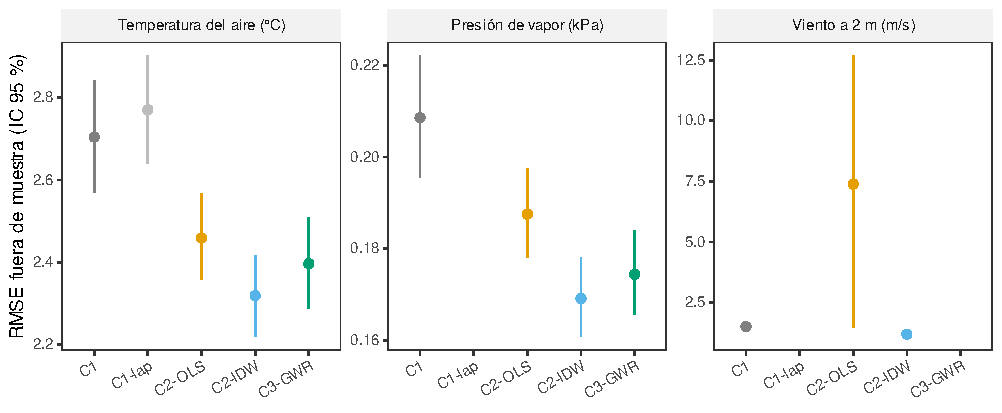
\includegraphics[width=\linewidth]{fig03_cv_rmse.pdf}
\caption{Error medio cuadrático fuera de muestra (IC~95\,\% por \emph{bootstrap} de días), validación cruzada espacial anidada de \NCVDays{} días. GWR del viento no fue factible; el gradiente de C1 solo se aplica a la temperatura.}\label{fig:cv}
\end{minipage}\hfill
\begin{minipage}[t]{0.40\textwidth}\centering
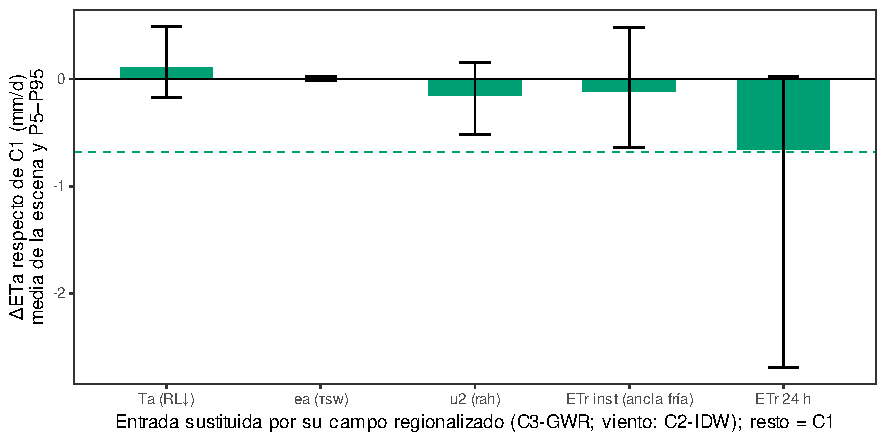
\includegraphics[width=\linewidth]{fig07_attribution.pdf}
\caption{Cambio de la $\ETa$ media al reemplazar una sola entrada de C1 por su campo regionalizado (GWR; viento: IDW). Barras: P5--P95 por celda. Línea discontinua: GWR completo.}\label{fig:attr}
\end{minipage}
\end{figure}
\begin{figure}[!htb]\centering
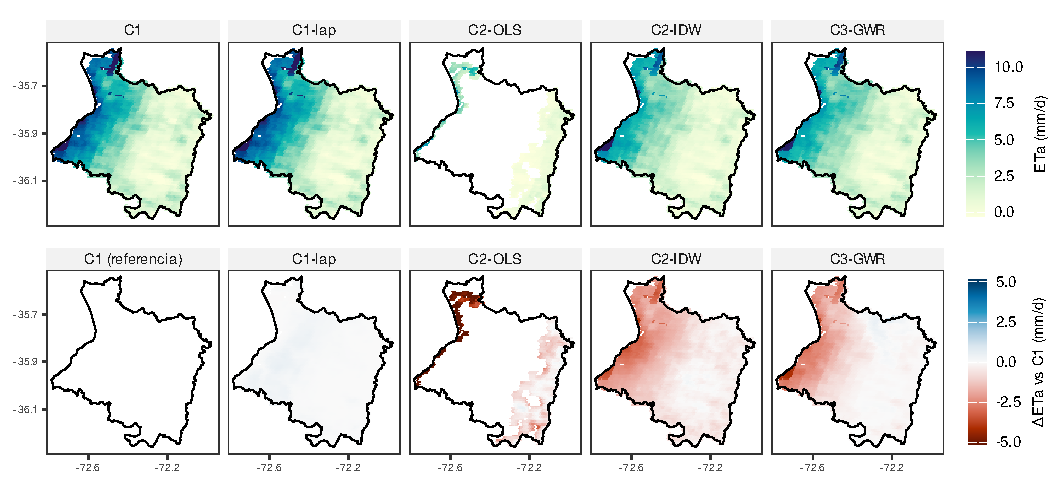
\includegraphics[width=0.70\textwidth]{fig06_eta_maps.pdf}
\caption{Arriba: evapotranspiración real diaria (mm/d) de la provincia de Cauquenes, 15 de febrero de 2019, por configuración. Abajo: diferencia respecto de C1. C2-OLS solo tiene datos donde el viento regionalizado quedó en el rango físico. Fuentes: MODIS C6.1, DMC, INIA, FDF, NOAA ISD, Copernicus GLO-90. Mostrado en WGS~84.}
\end{figure}
\end{document}
